% Chapter Template

\chapter{Methods} % Main chapter title

\label{Chapter2} % Change X to a consecutive number; for referencing this chapter elsewhere, use \ref{ChapterX}

%----------------------------------------------------------------------------------------
%	SECTION 1
%----------------------------------------------------------------------------------------

\section{Reynolds Number}

Our first goal is to find a set of points we will refer to as points of interests. To start we need to calculate the Reynolds-Number (\ensuremath{RE}) \ref{eq:1} of each voxel in every time step of the simulation. We take the product of \ensuremath{p,u} and \ensuremath{L} where \ensuremath{p} as the density of the fluid, \ensuremath{u} is the flow speed of the fluid, and \ensuremath{L} is the characteristic linear dimension. Then using the dynamic viscosity of fluid represented as $\mu$ as the divisor to get the \ensuremath{RE} for that voxel in that time-step. It should be noted that for constancy in our simulations \ensuremath{L} is calculated by calculating the average length of the sides of each voxel (\ensuremath{\sqrt[3]{l*w*h}}).  Due to this value being a constant in each calculation, changing this value can affect the discrete values obtained, but it does not alter the distribution of the values. 

\begin{equation}\label{eq:1}
RE  = \frac{puL} {\mu} 
\end{equation}

Now we have the Reynolds Number of every voxel in each time-step \ensuremath{RE_t} where \ensuremath{t} is an index number referencing a time value. Next we find the mean value for each voxel \ref{eq:2} then threshold the data into two categories; \ensuremath{RE>=150} as turbulent flow and \ensuremath{0<RE<=40} as laminar flow. We exclude \ensuremath{RE} values of zero because they are indicative of a voxel that is within an obstruction (e.g. underground, inside of a building). Next we need to compile a list of the index positions for the thresholded data and convert each set of indices to a 3-D point in space .
 \color{red} [Better way to state this?] \color{black} 
\begin{equation} \label{eq:2}
RE_{mean} = \frac{1}{n} \sum_{i=1}^{n} RE_{i}=\frac{1}{n}\left(RE_{1}+\cdots+RE_{n}\right)
\end{equation} 

We then run a clustering algorithm on each category of positions, in this case we use k-means due to its ease of implementation and speed when clustering large sets of points \cite{HDBScan}. This groups all points into \ensuremath{k} groups while minimizing the distance between a point and that group's centroid. We calculate the value of \ensuremath{k} by taking the \ensuremath{\frac{1}{2}\sqrt[3]{I*J*K}} where \ensuremath{I,J} and \ensuremath{K} are the number of voxels in the \ensuremath{x}, \ensuremath{y} and \ensuremath{z} axis respectively. We then are able to take the centroid from each cluster and  refer to these as our points of interest from now on. 


\begin{figure}
\centering
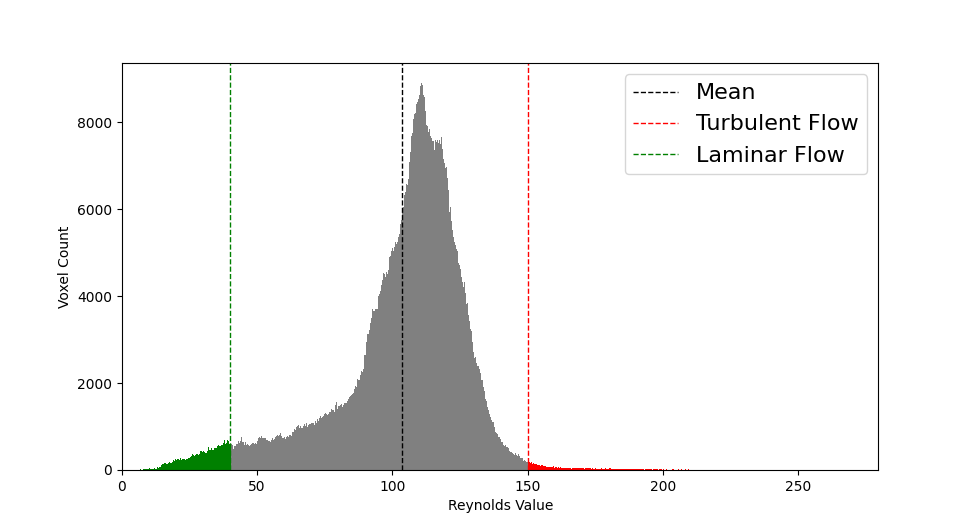
\includegraphics[scale=.35]{Figures/Hist4_11.png}
\decoRule
\caption[Reynolds Number Histogram]{Mean Reynolds Values Histogram}
\label{fig:MHistgram}
\end{figure}

\begin{figure}
\centering
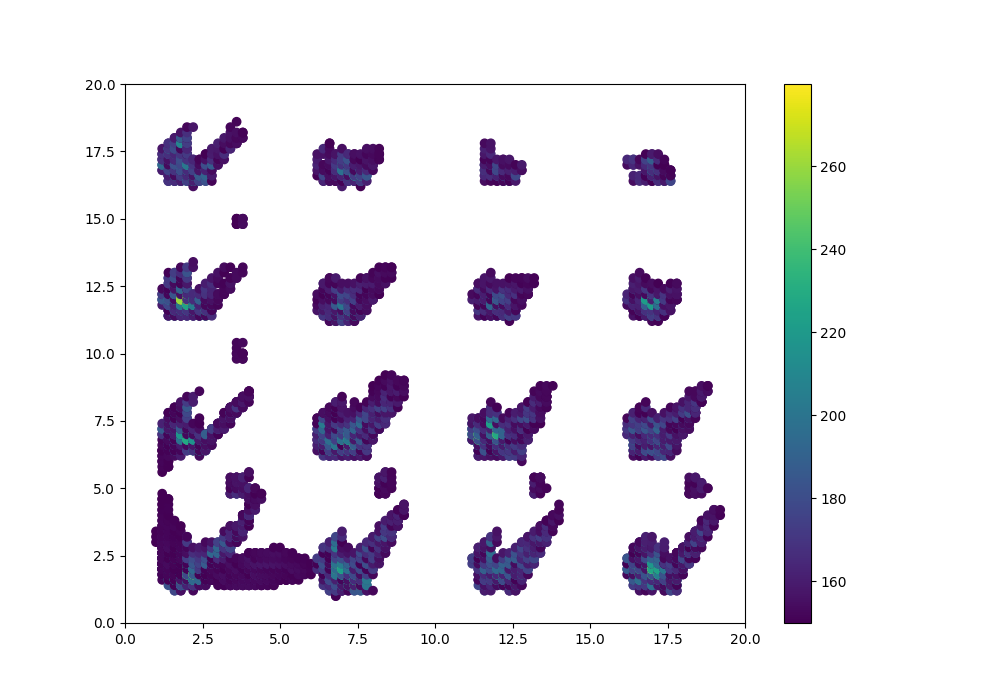
\includegraphics[scale=.35]{Figures/Turb2D_4_11.png}
\decoRule
\caption[Turbulent Air Flow Scatter Plot]{A top down view of a plot showing areas of turbulent air flow}
\label{fig:MTurbulentflow}
\end{figure}
%-----------------------------------
%	SECTION 2
%-----------------------------------
\section{Pathline Calculations}


Now that we have calculated these points of interest we can use an Ordinary Differential Equations (ODE) to calculate the streamlines. We will use a fifth-order Runge-Kutta method for adaptive time steps and to minimize errors in calculations. We are able to use forward and reverse integration to calculate path lines for every time step that passes through these points of interest. After integrating in both directions we then combine the posting and time data for each pathline while also adding in the Reynolds Number for each point as well. We store all of this data in hdf5 files so it can be quickly loaded into our visualization pipeline in Unity. 


%-----------------------------------
%	SECTION 3
%-----------------------------------
\section{Unity Visualization}
Once we read in all of the data for each point in each pathline into unity, we determine the largest (\ensuremath{RE_{max}}) and smallest (\ensuremath{RE_{min}}) value within the data set.  Now having the minimum and maximum values we are  able to calculate a color value for each segment of the pathlines. To do so we have to calculate the interpolant value within the range [\ensuremath{RE_{min}}, \ensuremath{RE_{max}}] \ref{eq:3}. TThis provides us with a value between [0,1] and then we can map this value to a color on a perceptually uniform color map \color{red} [We use  vega's magma color map with 8 colors] \color{black} For each time step we load in the respective data for all \ensuremath{k} pathlines. To resolve the issue of being able to see orientation but not true directionality of a pathline (a line going left to right looks identical to a line going right to left) we segment each pathline into n-1 line segments  (e.g. \ensuremath{P_0\rightarrow P_1},\ensuremath{P_1 \rightarrow P_2},...,\ensuremath{P_{n-2} \rightarrow P_{n-1}}).
We then adjust the starting width of each line segment to be the average length of a voxel and the ending width zero. This gives the lines a conical shape to indicate the directionality. We then build a color gradient texture and apply it to the texture from point to point with the precalculated color map. This resolves the issues with un-clear directionality in other visualization methods as previously discussed. We are able to compile and build our Unity system into an executable file that allows for the end user to run on any compatible system. We have the user interface (UI) designed to allow for viewing the simulation using a Head Mounted Display (HMD), a virtual reality headset, and controller or just a computer monitor with a keyboard and mouse for movement. Users just need to  type in the directory of the hdf5 files output discussed previously and the data is cashed for quick loading into the simulation. Then they are able to move around  the environment in either Virtual Reality or just by using the mouse and keyboard. 

\begin{equation} \label{eq:3}
f(RE_{min},RE_{max},RE_{value}) = \frac{RE_{value}-RE_{min}}{RE_{max}-RE_{min}}
\end{equation} 